%提出するレポートの書式はこのtemplateファイルに沿って作成してください。
%特に表紙・概要の書式は変えないで下さい。

\documentclass[a4j]{jarticle}

\usepackage[dvipdfmx]{graphicx}
\usepackage{epsbox}
\usepackage{url}
\usepackage{here}
\usepackage{ascmac}

\setlength{\headsep}{-5mm}
\setlength{\oddsidemargin}{0mm}
\setlength{\textwidth}{165mm}
\setlength{\textheight}{230mm}
\setlength{\footskip}{20mm}

\begin{document}



\section{モジュール設計}
\subsection{admin\_top.html}
\noindent
【名称】\\
管理者TOP画面\\
【概要】\\
管理者がログインを済ませると最初に現れる画面である。ここでは管理者に与えられた権限の選択をすることができる。\\
【処理フロー】
\begin{itemize}
\item 「掲示板はこちらボタン」を押すと、が呼び出される。
\item 「子管理者管理ボタン」を押すと、admin\_child\_top.htmlが呼び出される。
\item 「ユーザ管理ボタン」を押すと、が呼び出される。
\item 「お知らせ編集ボタン」を押すと、が呼び出される。
\item 「通報状況確認ボタン」を押すと、が呼び出される。
\item 「不適切な単語登録ボタン」を押すと、が呼び出される。
\end{itemize}

\subsection{admin\_child\_top.html}
\noindent
【名称】\\
子管理者管理TOP\\
【概要】\\
各子管理者について発行・抹消を行うための画面である。\\
【処理フロー】
\begin{itemize}
\item 「子管理者アカウント発行ボタン」を押すと、create\_admin.htmlが呼び出される。
\item 「子管理者抹消ボタン」を押すと、delete\_admin.htmlが呼び出される。
\item 「管理者TOPボタン」を押すと、admin\_top.htmlが呼び出される。
\end{itemize}

\subsection{create\_admin.html}
\noindent
【名称】\\
子管理者アカウント発行画面\\
【概要】\\
子管理者アカウントの発行を行うかどうかを決定する画面である。\\
【処理フロー】
\begin{itemize}
\item 「はいボタン」を押すと、.html.erbで処理が行われる。
\item .html.erbで新たなアカウントの発行が完了するとnew\_admin.htmlが呼び出される。
\item 「いいえボタン」を押すと、admin\_child\_top.htmlが呼び出される。
\end{itemize}

\subsection{new\_admin.html}
\noindent
【名称】\\
子管理者アカウント発行完了画面\\
【概要】\\
子管理者アカウント発行完了画面が表示される\\
【処理フロー】
\begin{itemize}
\item 「確認ボタン」を押すと、admin\_child\_top.htmlが呼び出される。
\item 「管理者TOPボタン」を押すと、admin\_top.htmlが呼び出される。
\end{itemize}

\subsection{delete\_admin.html}
\noindent
【名称】\\
子管理者アカウント抹消画面\\
【概要】\\
特定の子管理者アカウントについて抹消するかどうかを決定する画面である。\\
【処理フロー】
\begin{itemize}
\item 「はいボタン」を押すと、.html.erbで処理が行われる
\item .html.erbで子管理者アカウントの抹消が完了するとdelete\_admin\_ok.htmlが呼び出される。
\item 「いいえボタン」を押すと、admin\_child\_top.htmlが呼び出される。
\end{itemize}

\subsection{delete\_admin\_ok.html}
\noindent
【名称】\\
子管理者アカウント抹消完了画面\\
【概要】\\
子管理者アカウント抹消完了画面が表示される\\
【処理フロー】
\begin{itemize}
\item 「戻るボタン」を押すと、admin\_child\_top.htmlが呼び出される。
\end{itemize}

\subsection{user\_admin\_top.html}
\noindent
【名称】\\
ユーザ管理画面\\
【概要】\\
ユーザのアカウント発行とユーザ情報検索を行うことができる画面である。\\
【処理フロー】
\begin{itemize}
\item 「ユーザアカウント発行ボタン」を押すと、create\_user.htmlが呼び出される。
\item 「ユーザ情報検索ボタン」を押すと、search\_user.htmlが呼び出される。
\end{itemize}

\subsection{create\_user.html}
\noindent
【名称】\\
ユーザアカウント発行画面\\
【概要】\\
ユーザアカウントの発行を行うことができる画面である。学籍番号の開始番号と末尾番号を入力することで範囲を指定し、同時に複数のアカウントの発行を行う。\\
【処理フロー】
\begin{itemize}
\item 「開始番号テキストボックス」に新しく発行するユーザの開始番号を入力する。
\item 「末尾番号テキストボックス」に新しく発行するユーザの末尾番号を入力する。
\item 「登録ボタン」を押すと、.html.erbで処理が行われる。
\item .html.erbでユーザのアカウント発行が完了するとnew\_user.htmlが呼び出される。
\item 「管理者TOPボタン」を押すと、admin\_top.htmlが呼び出される。
\end{itemize}

\subsection{new\_user.html}
\noindent
【名称】\\
ユーザアカウント発行確認画面\\
【概要】\\
ユーザアカウント発行確認画面が表示される\\
【処理フロー】
\begin{itemize}
\item 「確認ボタン」を押すと、user\_admin\_top.htmlが呼び出される。
\end{itemize}

\subsection{search\_user.html}
\noindent
【名称】\\
ユーザ情報検索画面\\
【概要】\\
【処理フロー】
\begin{itemize}
\item 「学籍番号検索テキストボックス」にはユーザの情報を入手する際に学籍番号を入力する。
\item 「検索ボタン」を押すと、.html.erbで処理が行われる。
\item .html.erbで該当するユーザがあればuser\_info.htmlが呼び出される。
\end{itemize}

\subsection{user\_info.html}
\noindent
【名称】\\
ユーザ情報画面\\
【概要】\\
ユーザ情報の検索結果を表示する画面である。
【処理フロー】
\begin{itemize}
\item 「警告・注意喚起ボタン」を押すと、が呼び出される。
\item 「アカウント凍結ボタン」を押すと、が呼び出される。
\item 「パスワード表示ボタン」を押すと、が呼び出される。
\item 「管理者TOPボタン」を押すと、admin\_top.htmlが呼び出される。
\end{itemize}

\subsection{.html}
\noindent
【名称】\\
画面\\
【概要】\\
【処理フロー】
\begin{itemize}
\item 「ボタン」を押すと、が呼び出される。
\end{itemize}

\subsection{login\_top.html}
【名称】\\
ログインTOP画面\\
【概要】\\
利用者が本システムを利用する際の初期画面である。ここでは、ユーザとしてログイン、管理者としてログインのいずれかを選択することができる。\\
【処理フロー】
\begin{itemize}
  \item ログインボタンを押すとlogin\_user.htmlが呼び出される。
  \item 管理者はこちらボタンを押すとlogin\_admin.htmlが呼び出される。
\end{itemize}

%ユーザ側
\subsection{login\_user.html}
【名称】\\
ユーザログイン画面\\
【概要】\\
ユーザがIDとパスワードを入力して本システムにログインするための画面である。\\
【処理フロー】\\
\begin{itemize}
  \item 「ID入力テキストボックス」にユーザのIDを入力する。
  \item 「パスワード入力テキストボックス」にユーザのパスワードを入力する。
  \item 初回のログインでは、IDとパスワードが入力された状態で「ENTERボタン」を押すとsubscribe\_user.htmlが呼び出される。
  \item 2回目以降のログインでは、IDとパスワードが入力された状態で「ENTERボタン」を押すとBBS\_top.htmlが呼び出される。
  \item データベース上に存在しないIDまたはパスワードが入力された状態で「ENTERボタン」を押すと、.html.erbが呼び出される。
  \item いずれかのテキストボックスに何も入力されていない状態で「ENTERボタン」を押すと、.html.erbが呼び出される。
\end{itemize}


\subsection{subscribe\_user.html}
【名称】\\
新規登録画面\\
【概要】\\
初回ログインをしたユーザがIDとパスワードを変更し、本システムに本登録する画面である。\\
【処理フロー】\\
\begin{itemize}
  \item 「ID入力テキストボックス」に変更後のユーザIDを入力する。
  \item 「パスワード入力テキストボックス」に変更後のユーザのパスワードを入力する。
  \item 「パスワード再確認入力テキストボックス」に「パスワード入力テキストボックス」に入力したものと同じパスワードを入力する。
  \item 「ID」「パスワード」「パスワード再確認」のテキストボックスに文字列が入力されており、かつ「パスワード」と「パスワード再確認」のテキストボックスに入力された文字列が一致した場合において、「登録ボタン」を押すとsubscribe\_ok.htmlが呼び出される。
  \item いずれかのテキストボックスに何も入力されていない状態で「登録ボタン」を押すと、.html.erbが呼び出される。
  \item 「登録ボタン」を押したときに「パスワード」と「パスワード再確認」に入力された文字列が合致しなかった場合、.html.erbが呼び出される。
\end{itemize}


\subsection{subscribe\_ok.html}
【名称】\\
新規登録完了画面\\
【概要】\\
新規登録が完了したことを表示する画面である。\\
【処理フロー】\\
\begin{itemize}
  \item 「利用を開始するボタン」を押すと、BBS\_top.htmlが呼び出される。
\end{itemize}


\subsection{read\_news.html}
【名称】\\
お知らせ画面
【概要】\\
管理者からユーザに対するお知らせの詳細を表示する画面である。\\

%管理者側
\subsection{login\_admin.html}
【名称】\\
管理者ログイン画面\\
【概要】\\
管理者がIDとパスワードを入力して本システムにログインするための画面である。\\
【処理フロー】\\
\begin{itemize}
  \item 「管理者ID入力テキストボックス」に管理者のIDを入力する。
  \item 「管理者パスワード入力テキストボックス」に管理者のパスワードを入力する。
  \item 入力されたIDとパスワードがともにデータベースに登録されたものと合致している場合、「ENTERボタン」を押すとadmin\_top.htmlが呼び出される。
  \item 入力されたIDとパスワードのいずれかがデータベースに登録されているものと合致しない場合、「ENTERボタン」を押すと、.html.erbが呼び出される。
  \item IDとパスワードのいずれかが入力されていない場合、「ENTERボタン」を押すと、.html.erbが呼び出される。
\end{itemize}

\subsection{news\_edit.html}
【名称】\\
お知らせ編集画面\\
【概要】\\
管理者がユーザにお知らせを通達する内容を編集する画面である。\\
【処理フロー】\\
\begin{itemize}
  \item お知らせタイトル、内容に文字列が入力されている状態で「送信ボタン」を押すと、news\_edit\_confirm.htmlが呼び出される。
  \item お知らせタイトル、内容のいずれかに文字列が入力されていない状態で「送信ボタン」を押すと、.html.erbが呼び出される。
  \item 「管理者TOPボタン」を押すと、admin\_top.htmlが呼び出される。
\end{itemize}


\subsection{news\_edit\_confirm.html}
【名称】\\
お知らせ内容確認画面\\
【概要】\\
お知らせ編集画面で編集したお知らせ内容を確認する画面である。内容を確認し、送信するか否かを選択する。\\
【処理フロー】\\
\begin{itemize}
  \item 「はいボタン」を押すと、.html.erbが呼び出される。また、news\_edit\_ok.htmlが呼び出される。
  \item 「いいえボタン」を押すと、news\_edit.htmlが呼び出される。
\end{itemize}


\subsection{news\_edit\_ok.html}
【名称】\\
お知らせ作成完了画面\\
【概要】\\
お知らせの作成が完了したことを示す画面である。\\
【処理フロー】\\
\begin{itemize}
  \item 「戻るボタン」を押すとadmin\_top.htmlが呼び出される。
\end{itemize}

%検索画面
\subsection{search.html}
【名称】
\\検索結果画面
\\【概要】
\\利用者が検索を行った際に表示される画面。スレッドタイトルを押すとそのスレッドの閲覧画面が表示される。
\\【処理フロー】
\\\begin{itemize}
\item 「スレッドタイトル」を押すと、read\_thread.htmlを呼び出す。
\end{itemize}

%通報関係
\subsection{report\_reason.html}
【名称】
\\通報画面
\\【概要】
\\利用者が通報ボタンを押した際に表示される画面。
\\【処理フロー】
\\\begin{itemize}
\item 「理由テキストボックス」に通報する理由を入力する。
\item 「送信ボタン」を押すと、report\_confirm.htmlを呼び出す。
\end{itemize}
\subsection{report\_confirm.html}
【名称】
\\通報確認画面
\\【概要】
\\利用者が通報画面にて、「送信ボタン」を押した際に表示される。
\\【処理フロー】
\\\begin{itemize}
\item 「はいボタン」を押すと、report\_ok.htmlを呼び出します。
\item 「いいえボタン」を押すと、report\_reason.htmlを呼び出す。
\\\end{itemize}
\subsection{report\_ok.html}
【名称】
\\通報完了画面
\\【概要】
\\利用者が通報確認画面にて、「はいボタン」を押した際に表示される画面。
\\【処理フロー】
\\\begin{itemize}
  \item 「戻るボタン」を押すとcategory\_top.htmlを呼び出す。
\end{itemize}

%不適切な単語関連
\subsection{NGword.html}
【名称】
\\不適切な単語の登録画面
\\【概要】
\\管理者が掲示板において不適切な単語を登録する画面。「不適切な単語入力テキストボックス」に入力した
単語を「不適切な単語登録ボタン」を押すことで、不適切な単語として登録ができる。
表示されている単語の「削除ボタン」を押すことで、その単語を不適切な単語から外す。
\\【処理フロー】
\\\begin{itemize}
  \item 「不適切な単語入力テキストボックス」に単語を入力し、「不適切な単語登録ボタン」押すことで表示されて
  いる単語の一覧に入力された単語を追加し、(不適切な単語のデータベース)に追加する。
  \item 単語の「削除ボタン」を押すことで、不適切な単語の一覧からその単語を外し、(不適切な単語のデータベース)から外す。
\end{itemize}

\begin{figure}[H]
\begin{center}
\resizebox{8cm}{!}{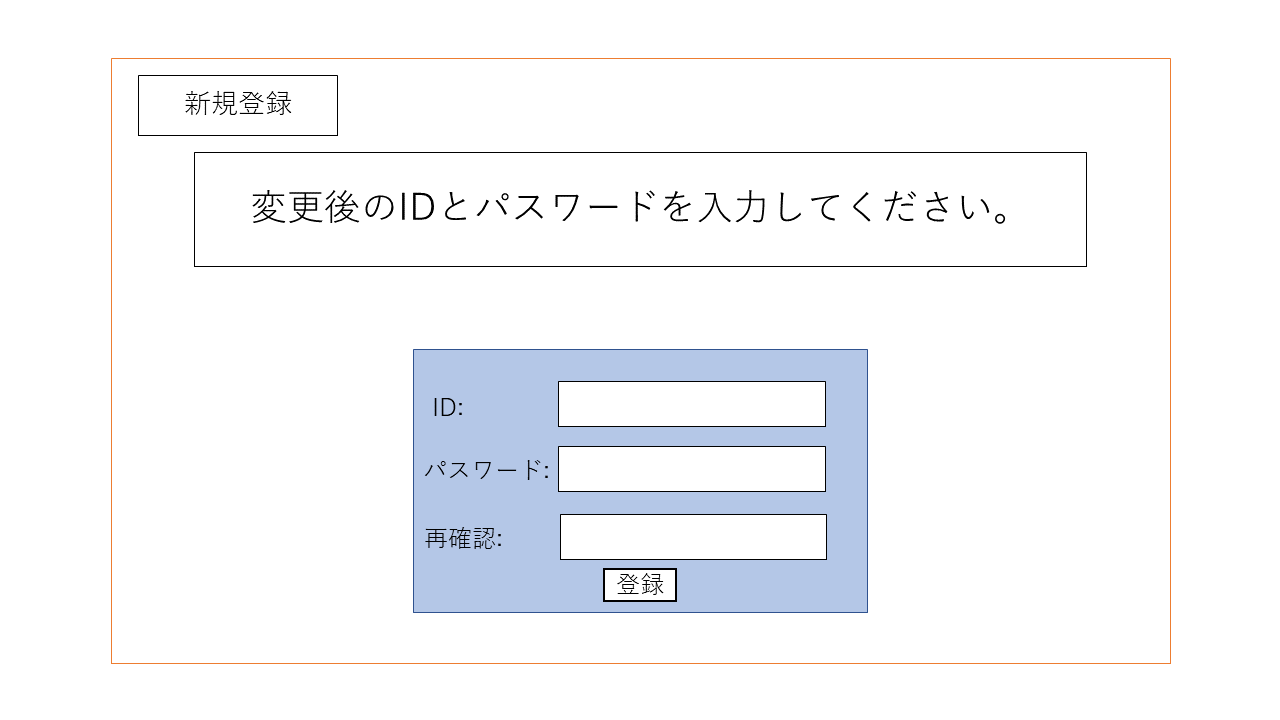
\includegraphics{sequence/subscribe_user.PNG}}
%\caption {カテゴリトップ画面}
%\label {fig:category\_top}
\end{center}
\end{figure}


\section{ルーティング及びMVC一覧}
この章では、Railsの規約に従ったURL規則を示す。また、HTTPメソッドとURLによって呼び出されるControllerとActionを示す。さらに、View及びModelも示す。
\newpage
\subsection{ルーティング一覧}
以下の表は、Railsの規則に従ったURL規則の表である。また、ControllerとそのActionについても示す。



\begin{table}[htb]
  \caption{ルーティング一覧}
  \centering
  \begin{tabular}{|l|l|l||l|} \hline
    No.&   URL 						&METHOD & Controller\#Action \\ \hline \hline
	 1&	/Login  					 	& GET      & sessions\#new       \\    
       2&  ~			         			& POST    & sessions\#create	\\
	 3&	/Logout   				      &DELETE   &sessions\#destroy	\\
	 4&	/passwords/:id					&GET	  &passwords\#new    \\
	 5 & /passwords/:id					&PATCH	  &passwords\#change \\
	 6&	/home   						& GET 	   &home\_pages/\#home    \\  
       7&	/home   						& PATCH 	   &home\_pages/\#threads\_hide \\   	               
	 8&	/users/:id     					&  GET  	    &  users\#show       \\      
	 9&	/users/:id     					 & PATCH   &  users\#update       \\               
	10&	/results/:title         			& GET   	    & results\#search      \\
	11& /results/:title/categories/:id		&GET		& categories\#search	\\
	12&	/informations/:id				  & GET       & informations\#show      \\
	13&	/categories/:id    		   		 &   GET      & categories\#index    \\
	14&	/threads/new      	 	  		 &  GET      &  threads\#new         \\
	15&/threads/check      		       &  GET      & threads\#check       \\
	16&/threads                   		       &  POST    &threads\#create      \\
	17&/threads/:id/report\_new   		&   GET      &threads\#report\_new  \\
	18&	/threads/check               		&   GET      & threads\#check       \\
	19&	/threads                      		 & POST     & threads\#create     \\ 
	20&	/threads/:id/contents      		 &    GET    & contents\#bbs        \\   
	21&	/threads/:id/contents/check 	&     GET    &  contents\#check   \\
	22&	/threads/:id/contents          	 &    POST  & contents\#write     \\
	23&	/threads/:id/contents          	 &    PATCH  & contents\#responses\_hide     \\
	24&	/threads/:id/contents/:id/report	 &    GET    & contents\#report    \\
	25&	/threads/:id/contents/:id/check   &   GET    &  contents\#check      \\
	26&	/threads/:id/contents            	 &   POST   & contents\#report\_create \\ \hline

\end{tabular}

\end{table}

\subsection{Controller}
\subsubsection{sessios\_controller.rb}
\noindent 名称:セッション情報処理	\newline
処理: \newline
-new:ログインフォームであるsessions\_new.html.erbを表示させる。\newline
-create:ユーザのIDとパスワードで認証を行い、認証されるとそのユーザのセッションを作成する。セッションを作成したユーザによって、以下のルーティングにリクエストを行う。\newline
ユーザが管理者:/adminに対してGETメソッドでルーティングにリクエストを行う。\newline
ユーザが一般ユーザ:/homeに対してGETメソッドでルーティングにリクエストを行う。また、そのユーザが初回ログインの場合は、/passwordsにGETメソットでルーティングにリクエストを行う。なお、認証が失敗した場合は再度/Loginに対してGETメソッドでルーティングを行う。\newline
-destroy:作成したユーザのセッションを破棄する。

\subsubsection{passwords\_controller.rb}
\noindent 名称:パスワード変更処理	\newline
処理:\newline
-new:初回ログインを行なった該当するユーザに対して、パスワード変更用フォームであるpasswords\_new.html.erbを表示させる。\newline
	-change:あらかじめ登録されていたユーザのパスワード情報を、変更用フォームから入力された新しいパスワードに更新する。更新後、/homeに対してGETメソッドでルーティングにリクエストする。

%'「該当する」という文言は、ユーザのidやスレッドのtitle等、DB上からなんらかの(一意な)属性の値を取得する処理が存在することを意味する



\subsubsection{home\_controller.rb}
\noindent 名称:ホーム画面処理 \newline
処理:\newline
-home:ホーム画面であるhome.html.erbを表示する。検索窓に検索したいスレッドタイトルを入力し、検索ボタンを押すと、/results/:idにGETメソッドでルーティングにリクエストを行う。お知らせを押すと、/infomations/:idにGETメソッドでルーティングを行う。マイページボタンを押すと、/user/:idにゲットメソッドでルーティングを行う。\newline

%管理者が推すと管理者ページへ戻る?


threads\_hide:不適切なスレッドを非表示化する。この処理は、管理者以外行うことはできない(非表示化ボタン自体が存在しない)。このアクションを行うと、/homeに対してPATCHメソッドでルーティングにリクエストする。



\subsubsection{users\_controller.rb}
\noindent 名称:マイページ画面処理 \newline
処理:\newline
-show:マイページ画面であるshow.html.erbを表示する。\newline
update:拡張機能を開放する(Userテーブルにおけるユーザの各種拡張フラグを1に更新する)アクションである。解放後、/user/:idにPATCHメソッドでルーティングにリクエストする。


\subsubsection{results\_controller.rb}
\noindent 名称:スレッドタイトル検索処理 \newline
処理:\newline 
-search:スレッドタイトル検索機能の処理を行うアクションである。検索を行い、該当するスレッドを取得した後は、そのスレッドを一覧として表示する(これがsearch.html.rbとなる)。表示されたスレッドタイトルを押すと、/threads/:id/contentsにGETメソッドでルーティングをリクエストする。\newline

\subsubsection{results\_categories\_controller.rb}
\noindent 名称:カテゴリ別スレッドタイトル検索処理 \newline
処理:\newline
search:スレッドタイトル検索機能の処理を行うアクションである。先ほど述べたスレッドタイトル検索処理とほとんど同じであるが、スレッドタイトル以外にも、該当するカテゴリであるかどうかを条件として検索を行う処理である。検索条件以外の処理に違いは存在しない。\newline



\subsubsection{infomations\_controller.rb}
\noindent 名称:お知らせ画面処理 \newline
処理:\newline
-show:お知らせ詳細画面であるshow.html.erbを表示する。\newline



\subsubsection{categories\_controller.rb}
\noindent 名称:カテゴリ別トップ画面処理 \newline
処理:\newline
-new:カテゴリ別トップ画面であるcategories.html.erbを表示する。この画面もトップ画面同様、検索窓が存在しているがこちらから検索を行うと、/results/:title/categories/:idにGETメソッドでルーティングをリクエストする。マイページに遷移するボタンの処理は、トップ画面と同様である。また、スレッドタイトルを押した場合は、/threads/:id/contentsにGETメソッドでルーティングをリクエストする。\newline



\subsubsection{threads\_controller.rb}
\noindent 名称:スレッド作成処理 \newline
処理:\newline
-new::スレッドを新規作成するフォームであるnew\_html.erbを表示させる。作成ボタンを押した後は/threads/checkにGETメソッドでルーティングをリクエストする。\newline
-check:スレッド作成確認画面であるcheck.html.erbを表示させる。確認ボタンを押すと、/thread/create\newline
-create:newアクションで入力されたスレッドタイトルと最初の書き込み内容を反映したスレッドを作成するアクションである。スレッドを作成した後は、カテゴリ別トップページである/categories/:idにGETメソッドでルーティングをリクエストする。


\subsubsection{contents\_controller.rb}
\noindent 名称:スレッド閲覧処理 \newline
処理:\newline
-bbs::スレッドを閲覧するページを表示するアクションである。通報ボタンを押すと、/thread/:id/contents/:id/reportにGETメソッドでルーティングをリクエストする。書き込みボタンを押すと、/thread/:id/contents/checkにGETメソッドでルーティングをリクエストする。\newline
-check:書き込み確認ページであるcontents\_check.html.rbを表示するアクションである。\newline
-write:threadに書き込みを行うアクションである。書き込み確認ページに存在する書き込みボタンを押すとこのアクションが実行され、その後/thread/:id/contents/にPOSTメソッドでルーティングをリクエストする。\newline
-responses\_hide:このアクションを実行できるのは管理者だけである。このアクションを実行すると、PATCHメソッドで/thread/:id/contentsにルーティングをリクエストする。\newline
-report:このアクションは、通報用フォームであるcontents.html.erbを表示させるアクションである。必要事項を入力し通報ボタンを押すと、通報確認ページである/thread/:id/contents/:id/checkにGETメソッドでルーティングをリクエストする。\newline
-check:通報確認ページであるcheck.html.erbを表示させるアクションである。\newline
-report\_create通報確認ページで確認ボタンを押すと、通報内容が作成される。その後、POSTメソッドで/thread/:id/contentsにルーティングにリクエストを行う。


\appendix

\end{document}
